% Report of the SS16 - X-ray Diffraction mini-project
% By Lyubomir Shoylev, 2022.
\documentclass[11pt,a4paper,twoside,onecolumn]{article}
\title{\textbf{SS16: X-ray diffraction and X-ray spectroscopy (mini-project)}}
\author{Lyubomir Shoylev, shil5377}
\date{\today}
% My report package :)
\usepackage{my-report}
\usepackage[default-range=1-1]{lipsum}
\newcommand{\reminder}[1]{\textcolor{red}{#1}}
\newcommand{\rydberg}{\mathrm{R}}
\newcommand{\Kalpha}{$\mathrm{K}_\alpha$~}
\newcommand{\Lalpha}{$\mathrm{L}_\alpha$~}

\begin{document}
\maketitle

\begin{abstract}
    \lipsum
\end{abstract}

\section{Introduction}

X-rays are an important experimental tool and have been for more than a 100 years now --- from the first Nobel Prize for their discovery, and still now. In this experiment, we will first verify Moseley's Law, and then use X-ray spectroscopy to analyse several samples of metal as well as coins from various places around the world.\reminder{finish this intro at the end.} %TODO

First, we examine some of the background theory behind X-rays and their production.

\subsection{X-ray atomic spectra}
The emission spectra of atoms is due to energy transition of shell electrons from a higher energy level to a lower energy level. We are interested in X-rays specifically, which are due to transitions in the inner electron levels. These are shielded from the outer electron layers (the higher $Z$, the better the shielding \reminder{CHECK}) and are mostly unaffected by the chemical structure of the sample i.e. by the surrounding atoms. Therefore, we can take an energy level of an electron to be $E_n = -\rydberg\left(Z\right) / n^2$ where $\rydberg = \rydberg_\infty \left(Z - b\right)^2$ is the modified Rydberg constant for a given $Z$, $b$ is some parameter, and $\rydberg_\infty$ is the hydrogen Rydberg constant. Then, the energy of an emitted photon by a transition from level $n_\mathrm{i}$ to $n_\mathrm{f}$ is given by:
\begin{equation}\label{eqn:x-ray-energy}
    \varepsilon = \rydberg\left(Z\right) \left(\frac{1}{n_\mathrm{f}^2} - \frac{1}{n_\mathrm{i}^2}\right).
\end{equation}
We can rewrite this at fixed $n_\mathrm{i}$, $n_\mathrm{f}$ (i.e. for a given line) as $\sqrt{\varepsilon} = m \times Z + C$ where $m$, $C$ are some constants. This relationship is known as `Moseley's Law'.

The names of the energy levels of low-$n$ in X-ray notation is described in table \ref{tab:x-ray-notation}. Usually, the lines which are due to an initial absence in level K1 are referred to K-series; similarly for L-series and so on.
\begin{table}[!htb]
    \centering
    \begin{tabular}{@{}cccccc@{}}
    \toprule
    \multicolumn{4}{l}{Quantum numbers} & \multirow{2}{*}{Atomic notation} & \multirow{2}{*}{X-ray notation} \\ \cmidrule(r){1-4}
    n      & l      & s       & j       &                                  &                                 \\ \midrule
    1      & 0      & 1/2     & 1/2     & 1S1/2                            & K1                              \\
    2      & 0      & 1/2     & 1/2     & 2S1/2                            & L1                              \\
    2      & 1      & 1/2     & 1/2     & 2P1/2                            & L2                              \\
    2      & 1      & 1/2     & 3/2     & 2P3/2                            & L3                              \\
    3      & 0      & 1/2     & 1/2     & 3S1/2                            & M1                              \\
    3      & 1      & 1/2     & 1/2     & 3P1/2                            & M2                              \\
    3      & 1      & 1/2     & 3/2     & 3P3/2                            & M3                              \\
    3      & 2      & 1/2     & 3/2     & 3D3/2                            & M4                              \\
    3      & 2      & 1/2     & 5/2     & 3D5/2                            & M5                              \\ \bottomrule
    \end{tabular}
    \caption{Table describing the connection between X-ray notation and Atomic notation. \reminder{cite source would be nice. Maybe add the old Siegbahn notation?}}
    \label{tab:x-ray-notation}
\end{table}

\subsection{X-ray production}\label{subsec:x-ray-production}
In practice, we produce X-rays by bombarding a sample of some material with high energy electrons or X-rays which removes one of the inner shell electrons from the sample atom. This produces a vacancy in the shell. The vacancy is filled by some electron of a higher $n$ orbit (see figure \ref{fig:emission-diagram}), and the fall of potential energy of the electron is compensated by an emitted X-ray (ignoring higher order effects like the \emph{Auger effect}).

\begin{figure}[!htb]
    \centering
    \includegraphics[width=\textwidth]{img/emission-diagram.png}
    \caption{Schematic of the emission process.}\label{fig:emission-diagram}
\end{figure}

Usually, small laboratory X-ray tubes use an electron source. Because of that, we observe a continuum of X-ray radiation imposed on top of the emission lines. This radiation is called \emph{bremsstrahlung} ("braking") radiation. Its source is the interaction between decelerating electrons and stationary charges in the sample lattice. The maximal energy of a bremsstrahlung continuum is limited by the energy of the decelerating particle. If electrons accelerated by a potential difference $V$, then the maximal energy is given by:
\begin{equation}
    \varepsilon_\mathrm{max} = eV
\end{equation}

Suppose we use one such continuous X-ray source for the production of X-rays form our sample. We will take the K-series as an example. To produce a vacancy, need an X-ray of energy $\varepsilon_\mathrm{in} = - E_1 = \rydberg(Z)$. The resultant energy of the emitted X-ray will be given by \eqref{eqn:x-ray-energy}. Take for example the K-L transition. Its energy will therefore be (ignoring fine-structure):
\begin{equation}
    \varepsilon_\mathrm{out} = \rydberg\left(Z\right) \left(1 - \frac{1}{2^2}\right).
\end{equation}
This is a process in which $\varepsilon_\mathrm{in} \neq \varepsilon_\mathrm{out}$, which is called \emph{flourescence}.

\subsection{Composition analysis}
As said above, the X-ray emission is relatively independent of the composition of the sample. We can use this fact to perform a composition analysis on a sample by exposing it to the continuous bremsstrahlung of a source; this will allow the different components to fluoresce. The signal will give us information not only \emph{which} elements are present (given that the source is high enough to allow fluorescence), but their relative contribution --- the intensity of the signal will depend only on the number density $n$. Suppose we measure the intensity of a two-metal alloy with the peaks in the K-L3 line as $I_\mathrm{a}$ and $I_\mathrm{b}$.
This tells us that:
\begin{equation}
    \frac{I_\mathrm{a}}{I_\mathrm{b}} = \frac{n_\mathrm{a}}{n_\mathrm{b}},
\end{equation}
where $n_\mathrm{a}$ and $n_\mathrm{b}$ are the number densities of materials a and b. From that, we could easily calculate percentage compositions for number densities or mass densities ($\rho = n \times (\text{molar mass})$).

\section{Experiment}
Our experiment consists of the following setup see figure \ref{fig:experim-setup}. First, we have an X-ray source with a molybdenum anode, which produces some characteristic \Kalpha X-rays that can be used for diffraction experiments (see the first experiment part of SS16 \reminder{put reference}) and some continuous bremsstrahlung (see section \ref{subsec:x-ray-production} for more details). These X-rays are focused through a circular aperture towards a target sample. The incident X-rays excite inner shell electrons, and the targets emit mostly in the characteristic X-rays of K,L, and M series. We detect these via an energy spectrometer that is sensitive in the region of our experiment. The setup parameters are: tube voltage $V = \SI{35}{kV}$, emission current \SI{1}{A}, exposure time $t=$\reminder{ask Darryl}. This allows us to produce X-rays from samples with atomic numbers \reminder{calculate}. These are a large part of the most commonly used materials in practice, e.g. copper.

\begin{figure}[!htb]
    \centering
    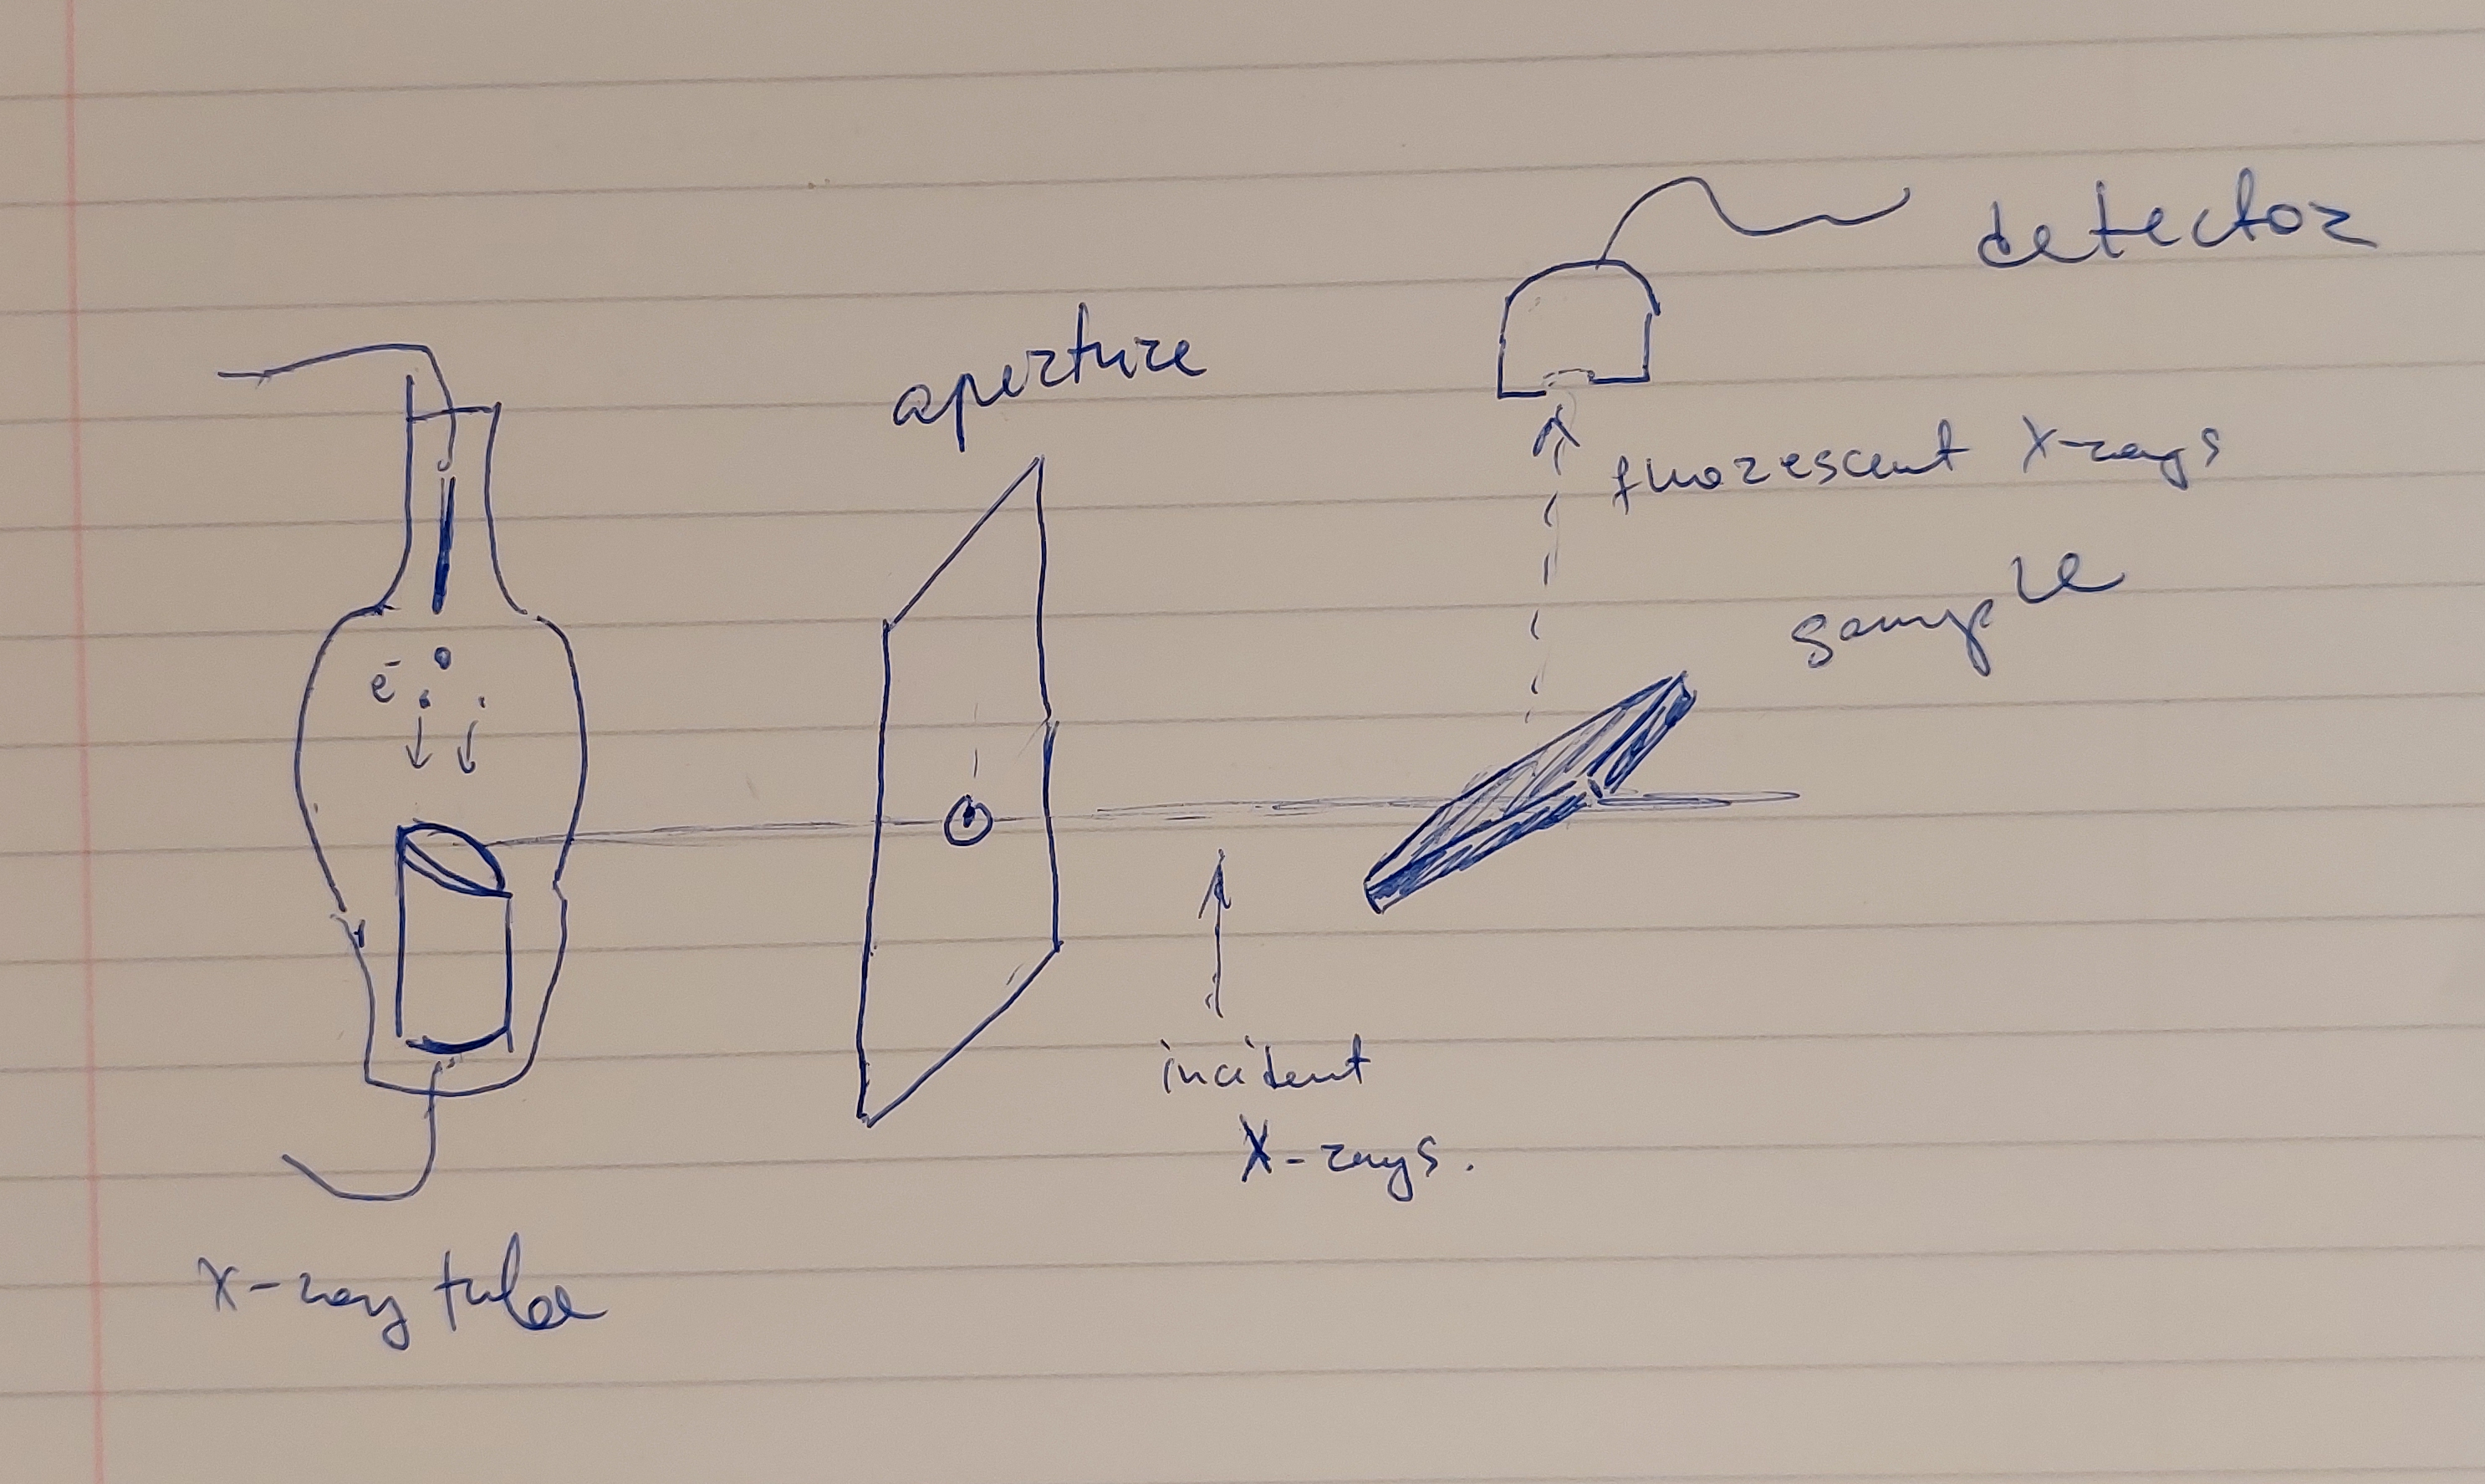
\includegraphics[width=\textwidth]{img/experim-setup.png}
    \caption{Diagram of the experimental setup. More info in the text of sec 2 }\label{fig:experim-setup}
\end{figure}

The first part of the experiment will test the validity of Moseley's Law with the help of several samples of known substances.

The second part and third part of the experiment will utilise our knowledge about X-rays to learn more about some samples provided for us, and about some metal coins from around the world.

\section{Result and Analysis}
Before we can do any work that has to do with determining energies or referring to energy values from a database, need to set the scaling of the measurement apparatus. We will do so with two of the labelled provided samples - for Fe and Ag. These cover a wide range of values in the bremsstrahlung spectrum, so they are a good way to set the scaling. The particular lines which we use to calibrate are the Fe \Kalpha with $E_\mathrm{Fe} = \SI{6.40}{keV}$ and the Ag \Kalpha with $E_\mathrm{Ag} = \SI{22.17}{keV}$.

\begin{figure}[!htb]
    \centering
    \includegraphics[width=0.5\textwidth]{img/calib.png}
    \caption{These are the Fe (black) and Ag (red) spectra used for calibration.}\label{fig:calibration}
\end{figure}

\subsection{Moseley's Law}
We measure the line energy values from the labelled samples. These are mainly in two groups:
\begin{itemize}[noitemsep]
    \item those, whose \Kalpha lines lie in the observable range (excluding our two calibration points);
    \item those, whose \Lalpha lines lie in the observable range.
\end{itemize}
We expect to see a straight line fit for the two groups of lines. The scaling constant $m$ depends purely on the line we are observing, i.e. on the $n_\mathrm{i}, n_\mathrm{f}$ for the given line. We can predict the ratio of the constants for the two series. Following \eqref{eqn:x-ray-energy} and Moseley's law, we get:
\begin{equation}
    m_\mathrm{K} \propto \left(1 - \frac{1}{2^2}\right)^{\sfrac{1}{2}} = \sqrt{\frac{3}{4}},\quad m_\mathrm{L} \propto \left(\frac{1}{2^2} - \frac{1}{3^2}\right)^{\sfrac{1}{2}} = \sqrt{\frac{5}{36}} \quad \Rightarrow \frac{m_\mathrm{K}}{m_\mathrm{L}} = \sqrt{\frac{27}{5}}
\end{equation}
\begin{figure}[!htb]
    \centering
    \includegraphics[width=0.8\textwidth]{img/moseleys.png}
    \caption{sqrt(energy) vs Z number for given samples: \reminder{list samples}.}\label{fig:moseleys}
\end{figure}


Results presented in figure \ref{fig:moseleys}.

We see that these both follow our expectations - have good fits to the model. We can deduce that our description of X-ray emission works sufficiently well for our purposes (given experimental accuracy etc), so we can proceed to use X-ray K and L series lines as a signature of a given element in spectral analysis.

Also, can calculate ratio from given values:
\begin{equation}
    \text{predicted: }\frac{m_\mathrm{K}}{m_\mathrm{L}} = \sqrt{\frac{27}{5}} = 2.324,\qquad \text{observed: } \frac{m_\mathrm{K}}{m_\mathrm{L}} = \frac{0.1026}{0.0411} = 2.496.
\end{equation}
Agreement is not so good, but we have not taken into account many other effects like change of energy due to being in a state $l \neq 0$ etc. So, not too bad. \reminder{can expand a bit maybe}.

\subsection{Provided alloys and semiconductors}
Now, can move to more interesting analysis. We will use the fluorescence to determine the composition of the semiconductors from the non-MP part and of some unlabelled samples that are provided in the physics lab.

\subsubsection{Semiconductors}
The semiconductors are part of the non-MP experiment, where we determined their structure by determination of the lattice constant. Here, we provide an independent confirmation of our previous results. 

\subsubsection{Unlabelled alloys}
The lab has two boxes of unlabelled metallic samples - alloys of different metals. We can determine their composition and ratios by using \reminder{ref 1.3}.

\subsection{International coins}
This is our final task. The lab has a box of various coins from around the world, the content of which we can again interpret using our fluorescence method.

The results can be summarised in the following table:
\reminder{include table for coins}
We can see that almost all coins are made of an alloy featuring Ni, Ci, or Zn. \reminder{discuss why}

\reminder{maybe additional analysis based on raw material cost of coins + a deeper inquiry?}

\section{Conclusions}
\lipsum[1-5]

\end{document}